% !TEX program = xelatex
% Aesthinema — making cinema under a consistency constraint.
% AC working draft. Companion artifact to the Asher Penn animation-pipeline
% correspondence: formalizes the continuity method, the wizard/approval
% tooling, the publishing surface, and the honest self-critique of the
% "safe register" these tools currently impose on the story.
\documentclass[10pt,letterpaper,twocolumn]{article}

% === GEOMETRY ===
\usepackage[top=0.75in, bottom=0.75in, left=0.75in, right=0.75in]{geometry}

% === FONTS ===
\usepackage{fontspec}
\usepackage{unicode-math}
\setmainfont{Latin Modern Roman}[
  Extension=.otf,
  UprightFont=lmroman10-regular,
  BoldFont=lmroman10-bold,
  ItalicFont=lmroman10-italic,
  BoldItalicFont=lmroman10-bolditalic,
]
\setsansfont{Latin Modern Sans}[
  Extension=.otf,
  UprightFont=lmsans10-regular,
  BoldFont=lmsans10-bold,
  ItalicFont=lmsans10-oblique,
  BoldItalicFont=lmsans10-boldoblique,
]
\setmonofont{Latin Modern Mono}[
  Extension=.otf,
  UprightFont=lmmono10-regular,
  ItalicFont=lmmono10-italic,
  Scale=0.85,
]

% === PACKAGES ===
\usepackage{xcolor}
\usepackage{graphicx}
\usepackage{booktabs}
\usepackage{tabularx}
\usepackage{caption}
\captionsetup{font=footnotesize, labelfont={bf}, labelsep=period}

% === AC LAYOUT (palette, fonts, watermark, sections, \ac, \code) ===
\usepackage{ac-paper-layout}
\graphicspath{{figures/}}

% additional AC color for the "holds" verdict
\definecolor{acgreen}{RGB}{74,120,74}

\hypersetup{
  pdftitle={Aesthinema — Making Cinema Under a Consistency Constraint},
  pdfauthor={@jeffrey},
}

% version stamp (regenerated by papers/cli.mjs on build; safe fallback here)
\InputIfFileExists{version}{}{\providecommand{\paperhash}{draft}\providecommand{\paperrev}{0}}

\begin{document}

% ==== TITLE BLOCK ====
\twocolumn[{%
\begin{center}
{\acbold\fontsize{34pt}{38pt}\selectfont Aesthinema\acdot}\par
\vspace{6pt}
{\large Making Cinema Under a Consistency Constraint}\par
\vspace{10pt}
{\normalsize\href{https://prompt.ac/@jeffrey}{@jeffrey}}\par
\vspace{3pt}
{\footnotesize\color{acgray} Aesthetic Computer \enspace$\cdot$\enspace Working Draft, July 2026}\par
\vspace{12pt}
\begin{minipage}{0.86\textwidth}
  \small\itshape
  These tools cannot hide one smell on their own: continuity. A face, a
  garment, a prop drifts from shot to shot, and the drift reads as the
  machine. This paper reports how that smell is fought inside a working,
  released body of generative media --- not with training or node graphs,
  but with three plain moves (canonical input imagery, descriptive text
  drawn from visual analysis, and director approvals), a small
  purpose-built ``wizard'' that keeps a human in the approval seat, and a
  set of ordinary hosted services stitched together in plain English. It
  also reports the uncomfortable part: right now the medium is shaping the
  story. What these tools can consistently produce quietly constrains what
  one can consistently \emph{tell} --- and a body of work made to survive
  that constraint has a recognizable, forgiving look. We name that look,
  trace how the pipeline was assembled over four months, catalog where its
  output is published, and mark the frontier where the constraint still
  binds.
\end{minipage}
\par\vspace{10pt}
\rule{\textwidth}{1.2pt}
\end{center}
\vspace{10pt}
}]

% ==== 1 THESIS ====
\section{The Smell Is Continuity}

Every generation is plausible in isolation. The failure is temporal: put
two frames of the same subject beside each other and the small
disagreements --- a collar that changes weave, a pen that migrates across a
pocket, a keyboard that becomes a typewriter --- announce that no single
thing was ever really \emph{there}. That announcement is the ``smell'' of
the tools. It is not removed by a better sampler or a larger model; it is
removed by pinning identity to something real and refusing to let it
wander.

The claim of this paper is narrower and more awkward than a method write-up
usually admits. The consistency problem is not only a production obstacle
to be engineered away. It is, today, an \emph{authorial constraint}. The
stories one can reliably tell with generative media are bounded by what the
medium can hold still. Work made honestly inside that boundary --- and the
released body described here was made honestly inside it --- inherits a
look: soft, bulky, forgiving, a little cartoon. Section~\ref{sec:safe}
names that look and argues it is partly a consistency strategy in
disguise. First, the moves that buy back as much continuity as the current
tools allow.

% ==== 2 THREE MOVES ====
\section{Three Moves}
\label{sec:moves}

No LoRA, no fine-tuning, no node editor. The method is three disciplines
applied in order, each one narrowing the space in which the model is free
to invent.

\paragraph{1. Canonical input imagery.} The model never invents the
subject. Every generation carries a fixed set of reference images of the
\emph{real} thing --- the actual person, the actual object --- so identity
is anchored to a photograph rather than to the model's imagination. In the
\ac{} portrait work this is a curated corpus of real photographs of the
subject; in client work it is the client's own drawings. The reference set
is not a suggestion appended to a prompt; it is the load-bearing element.
Elements pinned hard to a reference hold across a whole sequence. Elements
left to description alone wander (Section~\ref{sec:safe}).

\paragraph{2. Descriptive text from visual analysis.} One sits with the
ideal image and writes the subject down in obsessive, specific detail ---
not a vibe, the actual read of what is present. A prompt in this practice
does not say ``a pen.'' It says: \emph{``a yellow Sailor Pro Gear fountain
pen clipped into the shirt chest pocket, the clip hooked over the pocket's
top hem, the barrel tucked down inside so only the capped top stands above
the pocket.''} The closer the words track a real reference, the less room
the model has to drift. The description is authored against the canonical
imagery of Move~1, so the two reinforce: the picture pins the identity, the
words pin the read.

\paragraph{3. Director approvals.} Options per beat, a selection pass,
re-rolls on anything off-model, and nothing advances without a sign-off ---
the same loop one would run with a human animator. The difference is only
that generation makes the iterations cheap enough to actually run every
time. This is where the tooling lives (Section~\ref{sec:wizard}). The
approval seat is not automatable; it is the point.

% ==== 3 THE WIZARD ====
\section{The Wizards: Approval as Infrastructure}
\label{sec:wizard}

Move~3 is only real if sign-off is fast. The practice therefore carries a
small suite of native macOS applications --- informally, the ``wizards'' ---
each a purpose-built station in the pipeline: a clip wizard for auditioning
and picking motion takes, a shot wizard for laying out storyboards, a juke
wizard for rating and annotating the finished track library, and further
wizards for type and calendaring. They are real desktop apps, not web
pages; they share one sign-in and read the same on-disk conventions the
generators write, so approval sits in the pipeline as \emph{infrastructure}
rather than as an ad-hoc judgment made in a file browser.
Figure~\ref{fig:wizard} shows the clip wizard on one lane: the current
section, its take in a scrub player, the motion prompt that produced it, and
the keep/re-roll/assemble controls --- the approval gate as a native window.

\begin{figure}[t]
  \centering
  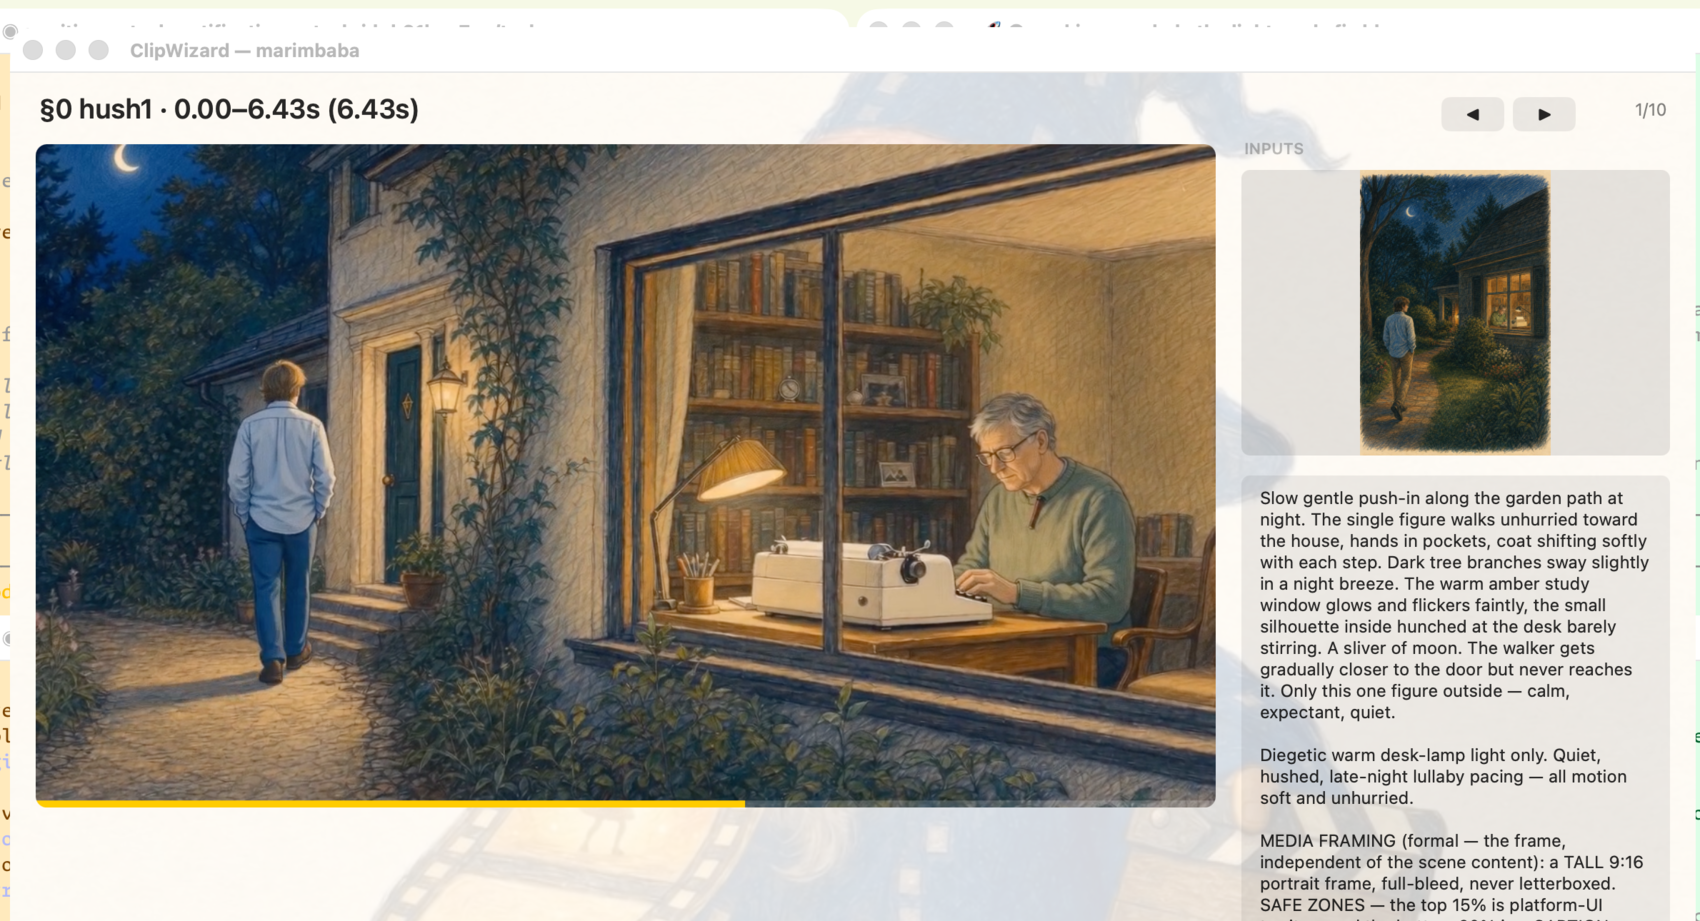
\includegraphics[width=\linewidth]{clipwizard.png}
  \caption{ClipWizard (native macOS) auditioning a lane's motion takes. Per
  section: the picked take in a scrub player, its generating prompt, and the
  keep / re-roll / assemble controls. Picking is free; only a re-roll spends
  money, and the old take is archived, never lost.}
  \label{fig:wizard}
\end{figure}

What the wizards operate on is a spread of candidates. Every beat is
generated several times over; Figure~\ref{fig:takes} shows four takes of a
single beat --- the same moment, the same subject, four framings. The
identity holds across all four (canonical imagery and description doing
their work); what differs is the \emph{read}, and choosing the read is the
director's job. The wizard is where one take is kept, the rest archived, and
anything off-model re-rolled --- the same loop one would run with a human
animator, made cheap enough to run on every beat. When the row is right, the
final cut is assembled \emph{from the picks}, without re-spending on shots
already owned.

\begin{figure}[t]
  \centering
  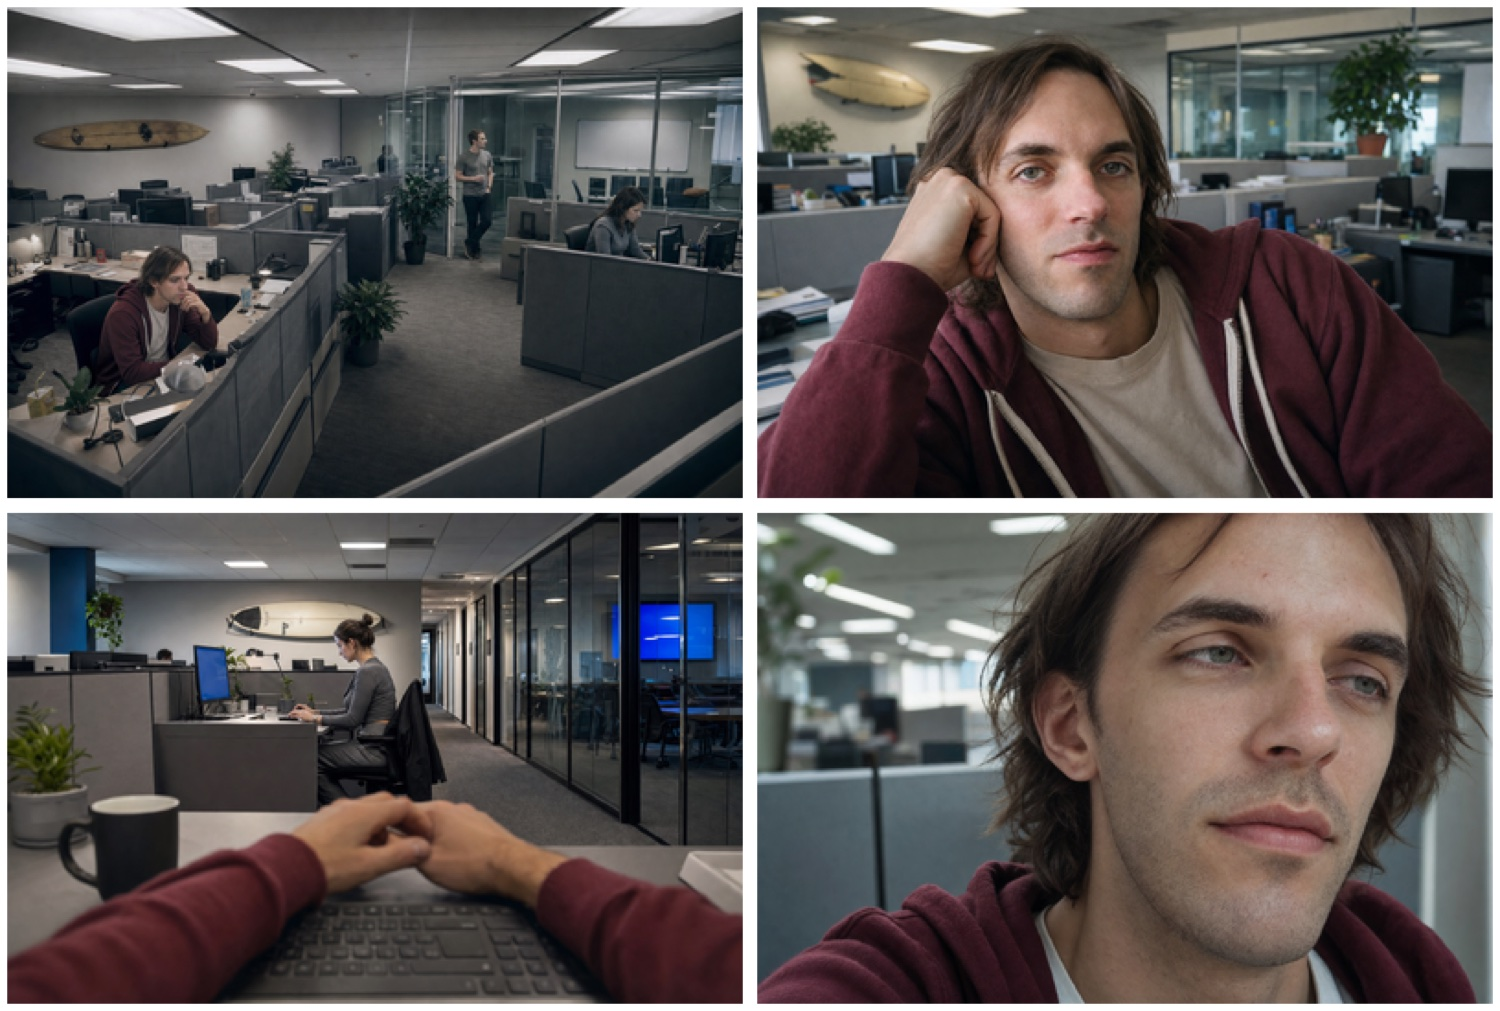
\includegraphics[width=\linewidth]{amay-takes.jpg}
  \caption{Four candidate takes of one beat (\emph{amaythingra}, opening ---
  the subject at his desk). Same moment, same subject, four framings; the
  likeness holds across all four. The wizard is where the director keeps one
  and re-rolls the rest --- options per beat, made cheap enough to judge
  every time.}
  \label{fig:takes}
\end{figure}

The node-graph tools popular for this work (ComfyUI and kin) offer real
capabilities the practice does not otherwise reach --- region/spot
treatment, painting a correction into one patch of a frame, and a visual
board of the whole pipeline. But granular control and a legible pipeline do
not require living in a node editor. The control that matters here is the
approval gate, and it is a native app pointed at the takes on disk.

% ==== 4 THE PIPELINE, DRAWN + PUBLISHED ====
\section{Plain English and Hosted Services}
\label{sec:pipeline}

The working method is, deliberately, boring: plain-English description plus
a handful of hosted services, stitched with a little glue code. Frames come
from \code{gpt-image-2} (OpenAI); motion from Seedance~2.0 (via
\code{fal.ai}); talking shots, when needed, from Kling AI Avatar; music,
notably, from \emph{no} model at all --- it is \ac{}'s own synthesis. There
is no training step and no node editor in the loop.

\begin{figure*}[t]
  \centering
  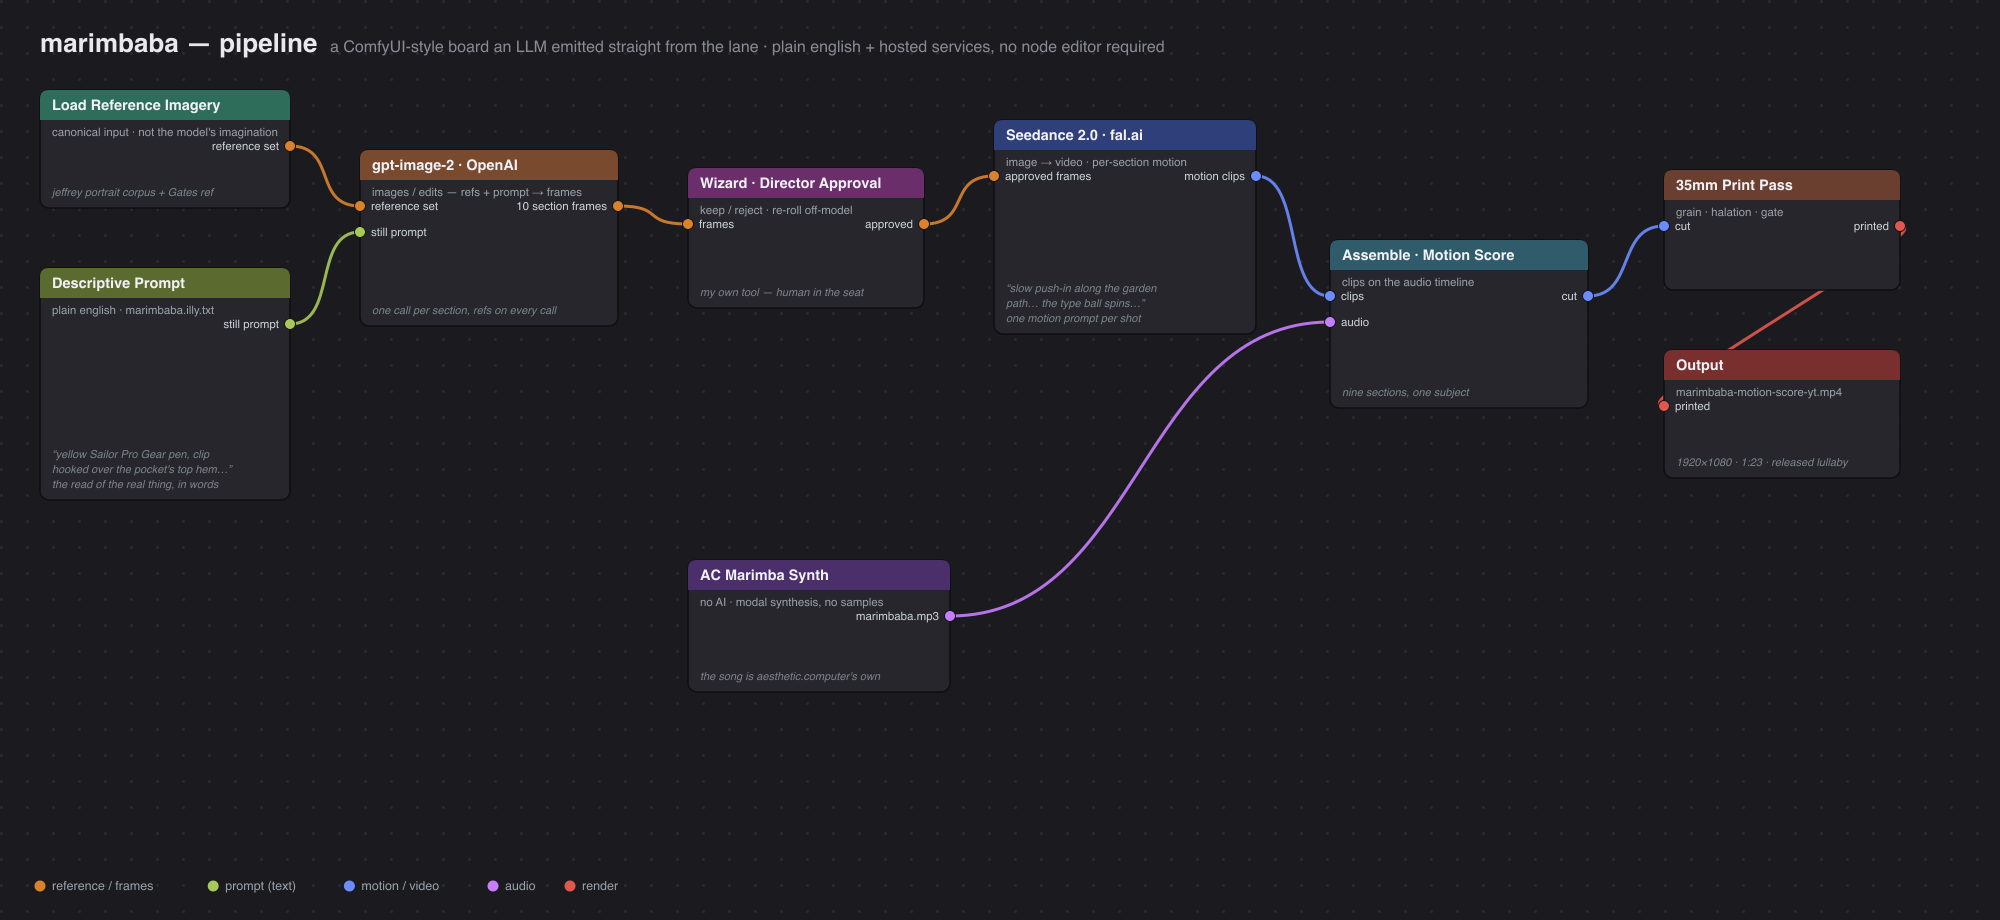
\includegraphics[width=0.92\textwidth]{comfy-board.png}
  \caption{The pipeline drawn as a node graph. This is not the practice
  working inside a node editor --- it is a diagram emitted from the lane's
  code in a single pass. The board is the easy part; the description and the
  approval seat are the parts that hold the work together.}
  \label{fig:board}
\end{figure*}

Figure~\ref{fig:board} makes a small point concretely. A director learning
a node tool partly to \emph{see} a pipeline can have that view for free: an
LLM will emit a chart or a node board directly from the pipeline it already
runs, shop the candidate services, and write the glue that stitches them ---
including, if one wants a starting point for something more elaborate, a
ComfyUI board to build on. The picture is cheap. The disciplines of
Section~\ref{sec:moves} are what is expensive, and what is worth keeping.

\paragraph{Where it goes out.} A pipeline is only a practice if its output
is published, and the surface here is broad and mostly automated
(Table~\ref{tab:endpoints}). Generative KidLisp source is minted to a short,
QR-able \code{\$code} URL; finished videos publish to two YouTube channels;
spoken-word ``readings'' of \ac{} essays --- voiced in a personal cloned
voice --- publish to Buzzsprout, which fans out to Spotify, Apple, and
YouTube; the voice itself is a cached service (\code{/api/say}); papers
publish as PDFs to a self-hosted index. Two surfaces remain deliberately
manual: the final DistroKid upload of a finished track, and Instagram /
TikTok posting. The through-line is that generative artifacts are not
demos; they are shipped, on named channels, on a schedule.

\begin{table}[t]
  \footnotesize
  \renewcommand{\arraystretch}{1.15}
  \begin{tabularx}{\linewidth}{@{}lXl@{}}
    \toprule
    \textbf{Surface} & \textbf{Publishes} & \textbf{Mode} \\
    \midrule
    \code{\$code}      & KidLisp source $\to$ short URL & auto \\
    YouTube            & videos, 2 channels            & auto \\
    Buzzsprout         & readings $\to$ Spotify/Apple  & auto \\
    \code{/api/say}    & cloned-voice TTS (cached)     & auto \\
    Papers             & PDFs $\to$ self-hosted index  & auto \\
    Bluesky            & posts                         & auto \\
    DistroKid          & finished tracks $\to$ Spotify & manual \\
    Instagram/TikTok   & reels, images                 & manual \\
    \bottomrule
  \end{tabularx}
  \caption{The generative-media publishing surface. Most of it is scripted
  from the repository; the two manual rows are marked as such.}
  \label{tab:endpoints}
\end{table}

% ==== 5 THE SAFE REGISTER ====
\section{The Safe Register}
\label{sec:safe}

Here is the honest part. The body of work a viewer sees first is the
\emph{safe} register --- the ``comfy'' output --- and its comfort is
partly engineered against the tools' failure mode. Three habits recur, and
each one is, read cynically, a consistency strategy:

\begin{itemize}
  \item \textbf{Soft, bulky materials.} Colored pencil on toothy paper,
  knit sweaters, needle-felted wool, gouache. A hand-drawn, broken-edged
  surface \emph{absorbs} the small spot errors that a crisp photographic
  surface would expose. The medium is chosen, in part, to forgive.
  \item \textbf{A cartoon space with familiar characters.} Cliché, legible
  figures in a warm, shallow set. Archetypes carry across frames on less
  description than a specific, grounded individual would demand.
  \item \textbf{Self-reflexive narratives.} Stories that are partly
  \emph{about} their own making, or about two figures in a small room, tend
  to forgive inconsistency the way a straight, grounded scene does not.
\end{itemize}

None of these is a cheat --- they are legitimate aesthetic choices, and the
work stands. But it is worth admitting that the aesthetic is downstream, in
part, of the constraint. To see the mechanism cleanly, consider one
released sequence.

\paragraph{Case study: \emph{marimbaba}.} A lullaby; two figures at a
late-night desk, nine sections, start to end (Figure~\ref{fig:frames}).
Across every section the elements pinned to canonical imagery and tight
description \emph{hold}: both faces, the red glasses-cords, the
blue-shirt/green-sweater split, the pens, the warm lamplit study. One
element was under-described --- the desk instrument. The prompt calls for a
specific IBM Model~M keyboard, but the reference was leaned on less there,
and the sequence keeps rendering it as a \emph{typewriter}; the smaller
desk props migrate shot to shot. That is the whole thesis in one image. The
elements pinned hard to a real reference held; the one described loosely
wandered. The fix is not a better model --- it is more canonical imagery and
tighter words, i.e.\ Section~\ref{sec:moves} applied harder.

\begin{figure}[t]
  \centering
  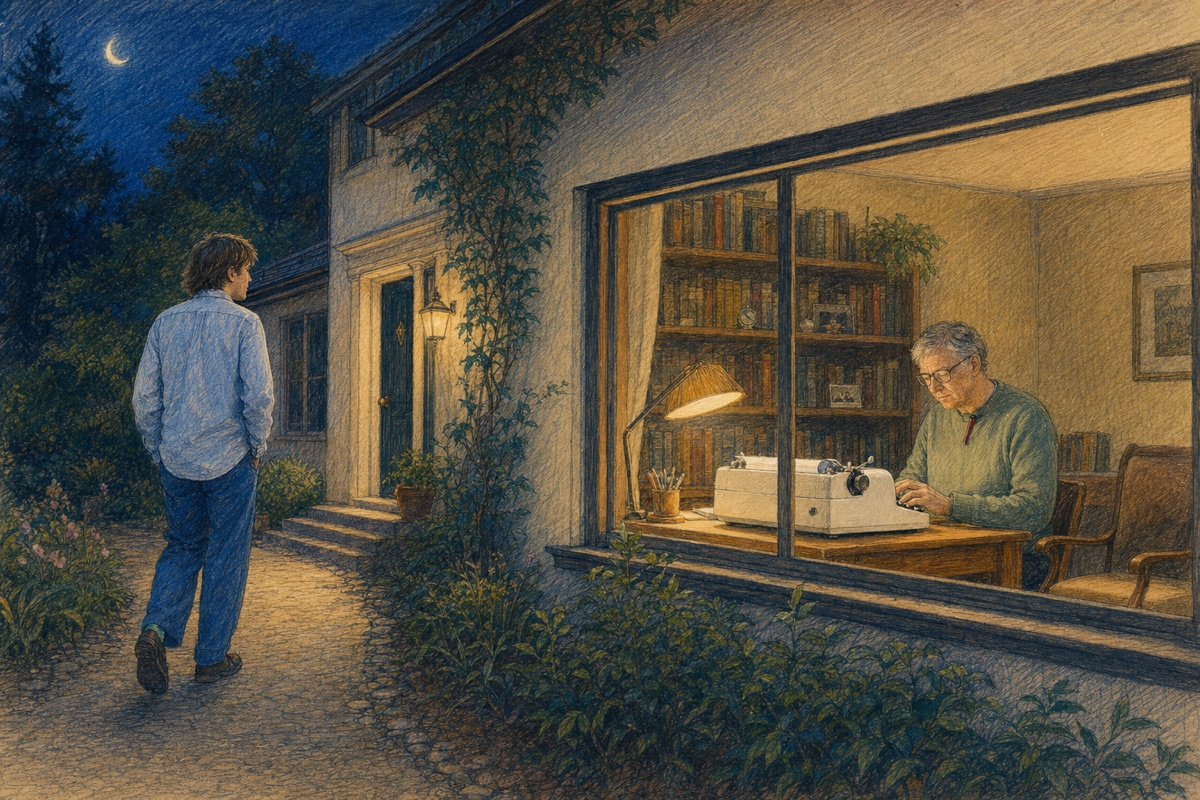
\includegraphics[width=0.485\linewidth]{frame-0-hush1.jpg}\hfill
  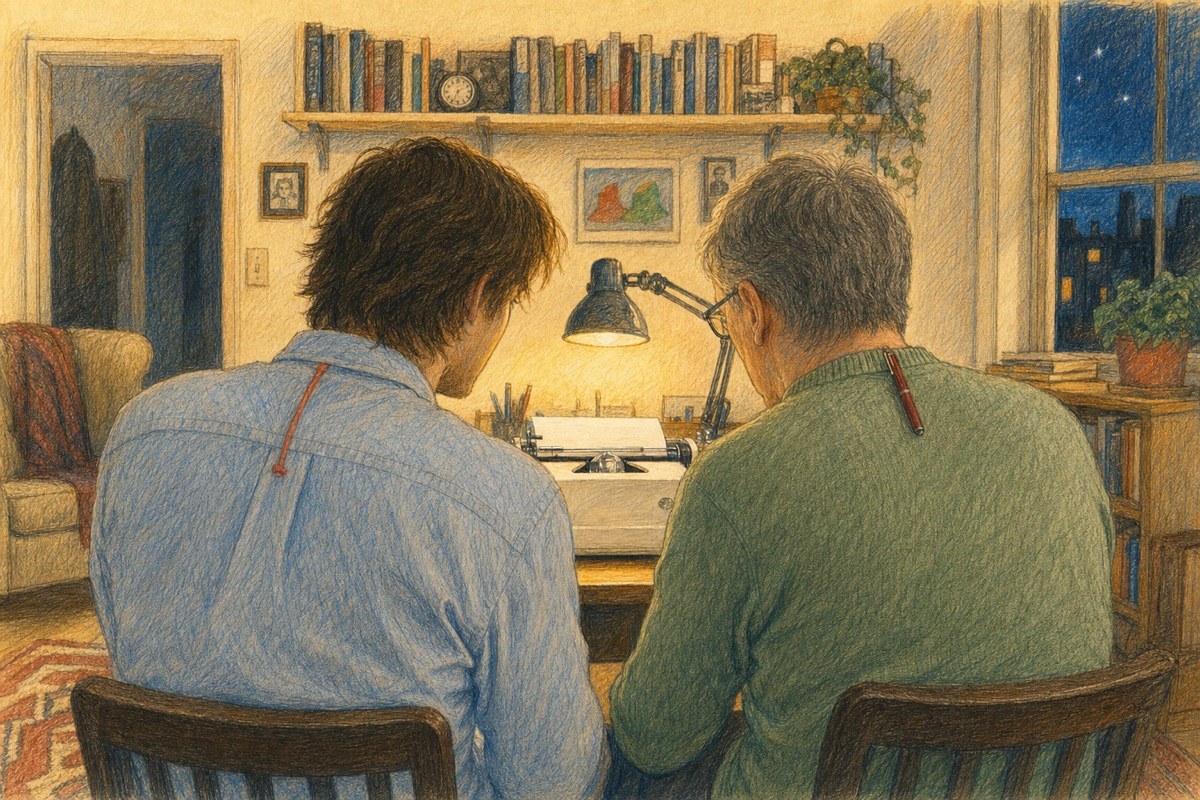
\includegraphics[width=0.485\linewidth]{frame-2-twinkle1.jpg}\\[3pt]
  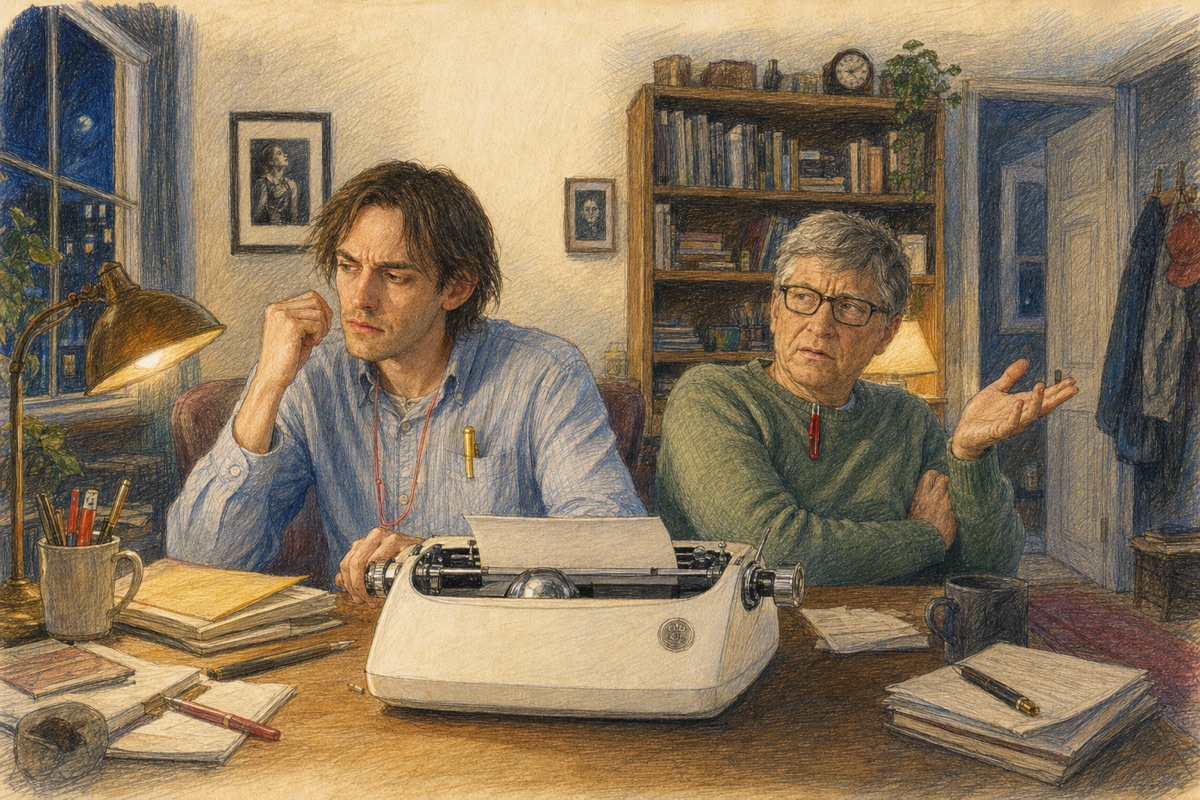
\includegraphics[width=0.485\linewidth]{frame-6-baba1.jpg}\hfill
  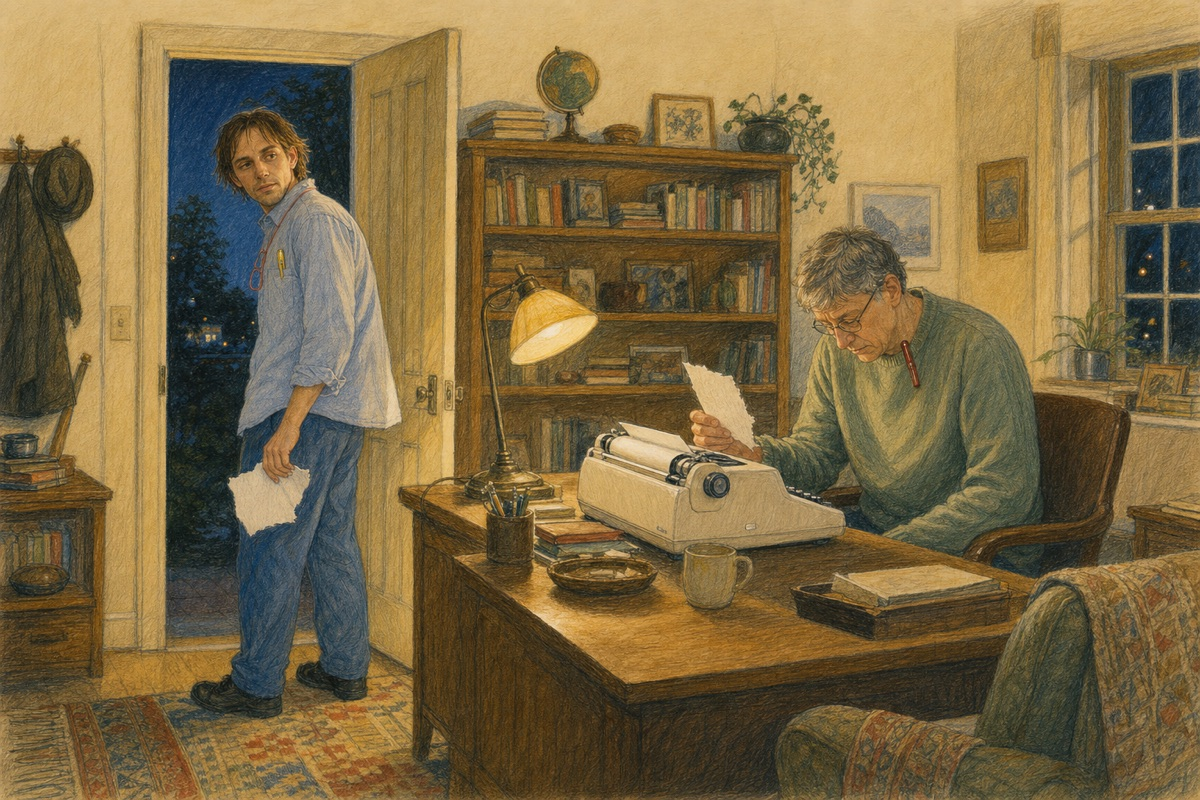
\includegraphics[width=0.485\linewidth]{frame-9-sleep2.jpg}
  \caption{\emph{marimbaba}, four of nine sections. The figures, cords,
  garments, and pens hold across the sequence (canonical imagery +
  description). The desk instrument --- under-described --- drifts toward a
  typewriter. \textcolor{acgreen}{What holds} was pinned;
  \textcolor{acpink}{what drifts} was merely described.}
  \label{fig:frames}
\end{figure}

\paragraph{Counter-case: \emph{amaythingra}.} The safe register is not the
only place the method works; it is only the cheapest. A second released
sequence pushes hard the other way. \emph{amaythingra} --- a deep-house
setting of \emph{Amazing Grace} --- renders a recognizable individual as a
glossy metaverse avatar and washes every frame in a single corporate
brand-blue color law (Figure~\ref{fig:amay}). Nothing here is soft or
forgiving: the render is crisp, sharp, and deliberately blur-free. The
continuity is bought two ways at once. The person is pinned to a reference
corpus and described in tight detail (Moves~1--2); and the single monotone
color grade does structural work --- a lane-wide color law is itself a
consistency device, fusing otherwise independent generations into one
world. The cost is exactly what the thesis predicts: more specificity on the
frame demands more canonical imagery and tighter words than the lullaby ever
did. It is the same discipline run with far less slack --- and it points
straight at the frontier (Section~\ref{sec:frontier}).

\begin{figure}[t]
  \centering
  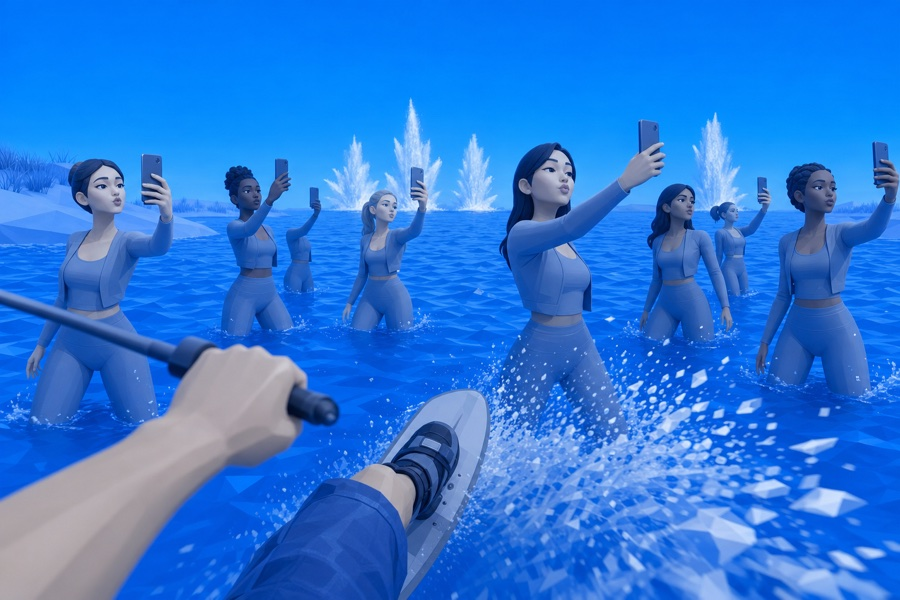
\includegraphics[width=\linewidth]{amay-vortex.jpg}
  \caption{\emph{amaythingra}: the crisp, specific register. A named subject
  as a low-poly avatar; a single Meta-blue (\#0668E1) color law over every
  frame doing double duty as satire and as a continuity device. The opposite
  of forgiving --- and it costs more description to hold.}
  \label{fig:amay}
\end{figure}

% ==== 6 STORYBOARD HISTORY ====
\section{A History of Storyboards}
\label{sec:history}

The method did not arrive whole; it accreted across a growing body of
storyboards --- roughly seventeen lanes to date --- each a small experiment
in how much continuity the current tools would grant. Every lane pairs the
same four artifacts: a descriptive still prompt (\code{*.illy.txt}, often
500--1500 words of camera, light, material, and mood), a scene or beat
script (\code{*.story.txt}), a per-section structure carrying figure and
face bounding boxes (\code{*-forms.json}, \code{*.struct.json}), and a
motion driver whose \code{SHOTS} table holds one 2--4 sentence choreography
per beat. Crucially the motion drivers \emph{inherit} the framing and
medium blocks from the still prompts (via a shared \code{mediums.mjs}), so
a single formal specification propagates from still to motion to release ---
one prompt genealogy per lane.

\begin{table}[t]
  \footnotesize
  \renewcommand{\arraystretch}{1.15}
  \begin{tabularx}{\linewidth}{@{}lXr@{}}
    \toprule
    \textbf{Lane} & \textbf{Shape} & \textbf{Sections} \\
    \midrule
    \emph{marimba}      & 24 pieces, 20 struct, 5 drivers & 4--34 \\
    \emph{momboba}      & epic + 3 reel variants          & 8--186 \\
    \emph{chillwave}    & landscape music video           & 73 \\
    \emph{americomputadora} & released single + canvas    & $\sim$8 \\
    \emph{comodiddies}  & numbered product reels          & per-beat \\
    whistlegraph-seedance & video-to-video, one rule      & per-clip \\
    campaigns           & 47 projects, 95 image prompts   & 1--26 \\
    \bottomrule
  \end{tabularx}
  \caption{A slice of the storyboard body. The most-developed lane,
  \emph{marimba}, spans two dozen character pieces and five motion drivers;
  the marketing campaigns alone hold ninety-five image prompts across
  forty-seven projects.}
  \label{tab:lanes}
\end{table}

The consistency lesson compounds across the set (Table~\ref{tab:lanes}).
The earliest lanes lean hardest on forgiving materials and faceless or
from-behind staging; the later lanes push more identity onto the frame and
pay for it with more canonical imagery and tighter description. The
whistlegraph-to-video work distills the whole discipline into a single
enforced rule --- \emph{graphics align with sounds} --- validated by frame
sampling and stroke counts before any motion is paid for.

% ==== 7 TIMELINE ====
\section{Four Months of Weaving}
\label{sec:timeline}

The pipeline was assembled in the open, one capability at a time, over
roughly four months. The trajectory is legible in the repository's history.

\begin{itemize}
  \item \textbf{March--April.} Music-first release tooling and the
  \emph{jeffrey-platter} --- the curated portrait/reference corpus that
  later anchors every stills deck (Move~1's raw material).
  \item \textbf{May.} Storyboard and score-to-media plumbing; the first
  ``wizard'' audition loops (a sing-wizard, then a wave-wizard); Spotify
  Canvas and YouTube publishing for singles.
  \item \textbf{June 11 --- the hinge.} The motion pipeline lands:
  descriptive illy storyboards $\to$ Seedance~2.0 motion, plus a clip
  wizard (\code{pop/lib/motion-pipeline.mjs}, \code{pop/lib/fal.mjs}). The
  same day, the first \emph{comodiddies} product (the 2FA Brush) ships as a
  full-motion reel. Within days a whole macOS wizard suite follows ---
  shot, juke, glyph, date --- unified under a shared sign-in.
  \item \textbf{June (rest).} Reel pipelines mature (\emph{marimbaba} 9:16,
  menuband promo, \emph{kidlisp-reels} with real 60\,fps GL capture);
  likeness-driven cinema via \code{gpt-image-2} stills decks and Ken Burns
  moves; grant concept films assembled from generated beauty shots.
  \item \textbf{July --- distribution and discipline.} A subscribable,
  personally-voiced podcast (essays $\to$ readings $\to$ Buzzsprout); the
  whistlegraph-to-Seedance workflow codified around ``graphics align with
  sounds,'' with cost-guarded storyboard validation before any video spend;
  and capture tooling (\emph{av-reels}) for real audiovisual performance.
\end{itemize}

The overall arc is a single lengthening chain --- \emph{synth track $\to$
storyboard $\to$ generated motion $\to$ chromed vertical reel $\to$
multi-channel release} --- growing more automated, more cost-aware, and more
unified under one identity and one wizard toolchain with each month.

% ==== 8 THE FRONTIER ====
\section{Where the Constraint Still Binds}
\label{sec:frontier}

The safe register is a real place to work, not a failure. But the frontier
is visible from it. The next demand is a story that will \emph{not} forgive
--- specific, grounded, consistent characters in a set that does not
absorb error, held across a long edit. That is where the marimbaba desk
instrument's drift stops being a charming imperfection and becomes the
whole problem. Nothing in the method changes at the frontier; it only has
to be applied with less slack: more canonical imagery, tighter description,
and an approval gate run on every panel before a frame is ever animated ---
sign-off first, motion second. The tools will keep improving underneath. The
disciplines are what travel.

\vfill
\begin{center}
  \footnotesize\color{acgray}
  Aesthetic Computer \; \textperiodcentered \; \texttt{aesthetic.computer} \\
  Working draft --- rev \paperrev\ (\paperhash)
\end{center}

\end{document}
